% L13a lecture companion. Notebook hashes and coverage are recorded in README.md.
% Style files and Cornell seal are copied unchanged from the L12c deck (identical
% to L12a, L10c, L10a, L9c, and L9a, which match the approved L6a deck). The
% six figures are the light TikZ PDFs in ../figs (Fig-Client-Server,
% Fig-HTTP-Messages, Fig-URL-Anatomy, Fig-JSON-Tree, Fig-REST-Cycle, and
% Fig-CRUD-Methods).
%
% Terms follow the lecture: web service, API, client, server, endpoint, the four
% parts of a request (method, URL, headers, body), the three parts of a response
% (status code, headers, body), JSON objects, arrays, and values, resource, the
% four-step request-response cycle, CRUD, and safe and idempotent methods.
\documentclass[aspectratio=169,11pt]{beamer}
\usepackage{vnslides}
\renewcommand{\vnlecturecode}{L13a}
\newcommand{\lecturelink}{https://github.com/varnerlab/CHEME-5800-CourseRepository-Fall-2026/blob/main/weeks/week-13/L13a/CHEME-5800-L13a-Lecture-RESTJSONAndSchemas-Fall-2026.ipynb}
\newcommand{\examplelink}{https://github.com/varnerlab/CHEME-5800-CourseRepository-Fall-2026/blob/main/weeks/week-13/L13a/CHEME-5800-L13a-Example-RESTful-NWS-Fall-2026.ipynb}
\newcommand{\lecturesource}[1]{\note{[Sources]\par
  \href{\lecturelink}{L13a lecture: RESTful Web Services and APIs.}\par
  #1\par[/Sources]}}
\newcommand{\code}[1]{\texttt{#1}}

\title{\texorpdfstring{{\vnheavy L13a}: RESTful Web Services and APIs}{L13a: RESTful Web Services and APIs}}
\subtitle{\texorpdfstring{HTTP requests, responses, and the CRUD methods\\[3pt]CHEME 5800 Cornell University}{HTTP requests, responses, and the CRUD methods; CHEME 5800 Cornell University}}
\author{Copyright Jeffrey Varner 2026. All Rights Reserved}

\begin{document}
\special{pdf:minorversion 7}
\vntitlepage

\begin{frame}{Objectives for Today}
  How does our code get data from a program that runs on another computer?

  \vspace{0.4em}
  {\large\textbf{\ink{Today's concepts}}}
  \vspace{0.2em}
  \begin{itemize}\setlength{\itemsep}{0.4em}
    \item \hilite{Describe web services and APIs}: a web service lets machines
      interact over a network, and an API is the set of rules used to access
      the service.
    \item \hilite{Read an HTTP request and response}: a request has a method, a
      URL, headers, and a body. A response has a status code, headers, and a
      body.
    \item \hilite{Explain how a RESTful API works}: follow a request through a
      RESTful web service, and map the create, read, update, and delete
      operations onto the HTTP methods.
  \end{itemize}
  \slidenote{Lecture:}{\href{\lecturelink}{RESTful Web Services and APIs}}
  \lecturesource{Introduction and three Learning Objectives.}
\end{frame}

\begin{frame}{Lecture and Example}
  \textbf{\ink{Lecture:}}
  \href{\lecturelink}{RESTful Web Services and APIs}

  In this lecture, we introduce web services and the application programming
  interfaces (APIs) that our programs use to call them. We focus on RESTful
  APIs, the most common design for web services, and on the HTTP methods that
  create, read, update, and delete data.

  \vspace{1.1em}
  \textbf{\ink{Example:}}
  \href{\examplelink}{Download a weather forecast from the National Weather Service API}

  In this example, we write a small Julia library, called a software
  development kit (SDK), for the RESTful API of the National Weather Service.
  We make HTTP GET calls to two endpoints and return the hourly forecast for
  Ithaca, NY as a table.
  \lecturesource{Introduction and the Examples section.}
\end{frame}

\begin{frame}{Web Services and APIs}
  A \hilite{web service} is software that lets machines interact over a
  network. The \hilite{client} makes a request, and the \hilite{server}
  answers it.

  \vspace{0.5em}
  \centering
  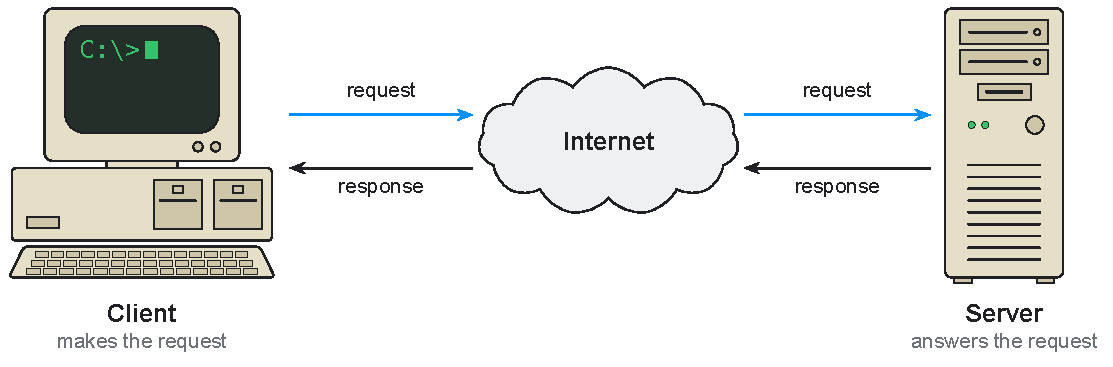
\includegraphics[width=\textwidth,height=0.52\paperheight,keepaspectratio]{assets/Fig-Client-Server.pdf}
  \lecturesource{Web Services and APIs: the opening definitions and the client and server figure.
    Figure: ../figs/Fig-Client-Server/Fig-Client-Server.pdf (light TikZ build).}
\end{frame}

\begin{frame}{APIs and Communication Protocols}
  An \hilite{application programming interface (API)} is the set of rules
  used to access the service.

  \vspace{0.3em}
  \begin{itemize}\setlength{\itemsep}{0.4em}
    \item \hilite{API specification}: the requests that a client can make and
      the data that comes back.
    \item \hilite{Communication protocol}: a shared set of rules for exchanging
      messages. Most web services use the Hypertext Transfer Protocol (HTTP),
      with data in formats such as JSON, CSV, and XML.
  \end{itemize}

  \vspace{0.4em}
  HTTP messages usually travel over TCP, which delivers the bytes reliably and
  in order. Almost every public API requires HTTPS, which is HTTP sent over a
  connection encrypted with Transport Layer Security (TLS).
  \lecturesource{Web Services and APIs: the API definition, the API specification, the communication protocol, and the TCP and HTTPS paragraph.}
\end{frame}

\begin{frame}{A Request and Its Response}
  HTTP is a \hilite{request-response} protocol. The client sends a request
  message, and the server answers with a response message.

  \vspace{0.5em}
  \centering
  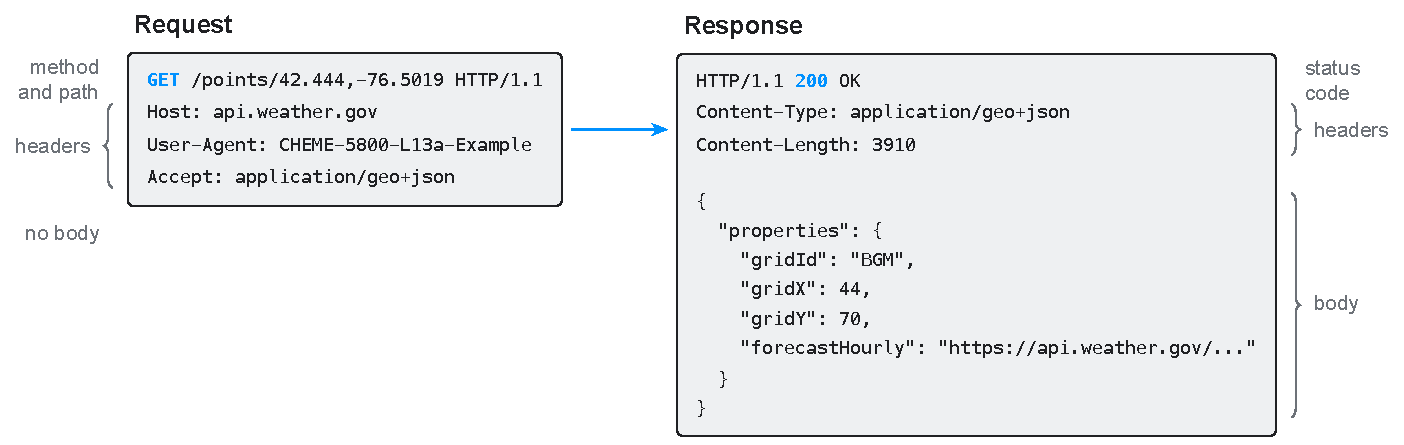
\includegraphics[width=\textwidth,height=0.46\paperheight,keepaspectratio]{assets/Fig-HTTP-Messages.pdf}

  \vspace{0.5em}
  \raggedright
  A client asks the National Weather Service (NWS) API for the data that it
  holds about Ithaca, NY. The status code \code{200} says that the request
  succeeded.
  \lecturesource{HTTP Requests and Responses: the opening paragraphs and the request and response figure.
    Figure: ../figs/Fig-HTTP-Messages/Fig-HTTP-Messages.pdf (light TikZ build).}
\end{frame}

\begin{frame}{The HTTP Request}
  A request has four parts:
  \begin{itemize}\setlength{\itemsep}{0.6em}
    \item \hilite{Method}: a verb that says what the client wants to do with
      the data, e.g., \code{GET} to retrieve it.
    \item \hilite{Headers}: name and value pairs that describe the request,
      e.g., the \code{User-Agent} header identifies the client, and the
      \code{Accept} header gives the data format that the client wants.
    \item \hilite{Body}: the data that the client sends to the server. The
      body is optional, and the \code{GET} requests in this lecture do not
      send one.
    \item \hilite{URL}: the Uniform Resource Locator, the address of the data
      on the server.
  \end{itemize}
  \lecturesource{The Request: the method, the headers, the body, and the URL.}
\end{frame}

\begin{frame}{The Pieces of a URL}
  A URL has four main pieces.

  \vspace{0.6em}
  \centering
  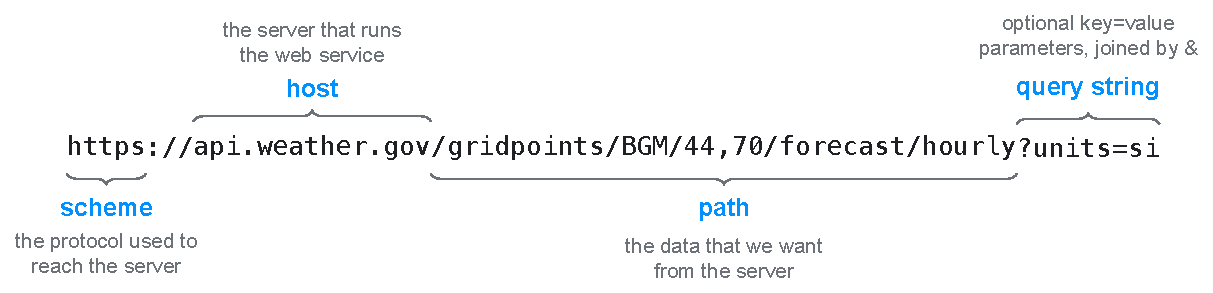
\includegraphics[width=\textwidth,height=0.44\paperheight,keepaspectratio]{assets/Fig-URL-Anatomy.pdf}

  \vspace{0.6em}
  \raggedright
  The URLs that an API publishes are called \hilite{endpoints}. The NWS API
  has one endpoint for the data about a location, and another endpoint for an
  hourly forecast.
  \lecturesource{The Request: the URL figure and the definition of an endpoint.
    Figure: ../figs/Fig-URL-Anatomy/Fig-URL-Anatomy.pdf (light TikZ build).}
\end{frame}

\begin{frame}{The HTTP Response}
  A response has three parts: a \hilite{status code}, the \hilite{headers},
  and the \hilite{body}. The first digit of the status code gives the class of
  the response:

  \vspace{0.2em}
  \centering
  {\small\setlength{\tabcolsep}{6pt}%
  \begin{tabular}{>{\raggedright\arraybackslash}p{0.09\textwidth}>{\raggedright\arraybackslash}p{0.30\textwidth}>{\raggedright\arraybackslash}p{0.50\textwidth}}
    \toprule
    \textbf{Class} & \textbf{Meaning} & \textbf{Common codes}\\
    \midrule
    \code{2xx} & the request succeeded & \code{200 OK}, \code{201 Created}, \code{204 No Content}\\
    \addlinespace
    \code{3xx} & the client must take another step & \code{301 Moved Permanently}\\
    \addlinespace
    \code{4xx} & the client made an error & \code{400 Bad Request}, \code{401 Unauthorized}, \code{403 Forbidden}, \code{404 Not Found}, \code{429 Too Many Requests}\\
    \addlinespace
    \code{5xx} & the server failed & \code{500 Internal Server Error}, \code{503 Service Unavailable}\\
    \bottomrule
  \end{tabular}}

  \vspace{0.3em}
  \raggedright
  A \code{4xx} code means that the problem is with the request that the client
  sent. A \code{5xx} code means that the server could not process it.
  \lecturesource{The Response: the status code, the headers, the body, the status code table, and the paragraph after it.}
\end{frame}

\begin{frame}{JSON}
  \hilite{JavaScript Object Notation (JSON)} is a text format for structured
  data. Most web services use JSON for the body of a request and the body of a
  response.

  \vspace{0.3em}
  \begin{itemize}\setlength{\itemsep}{0.5em}
    \item \hilite{Object}: a set of \code{"key": value} pairs inside braces
      \code{\{ \}}.
    \item \hilite{Array}: an ordered list of values inside brackets
      \code{[ ]}.
    \item \hilite{Value}: a string, a number, \code{true}, \code{false},
      \code{null}, or another object or array.
  \end{itemize}

  \vspace{0.4em}
  \hilite{Parsing} converts JSON text into data that a program can use. In
  our Julia code, a parsed object becomes a dictionary and a parsed array
  becomes a vector. \hilite{Serialization} converts the data in a program into text such
  as JSON.
  \lecturesource{JSON: the definition, objects, arrays, and values, and parsing and serialization.}
\end{frame}

\begin{frame}{JSON Text Is a Tree of Data}
  Each line out of an object carries a key.

  \vspace{0.6em}
  \centering
  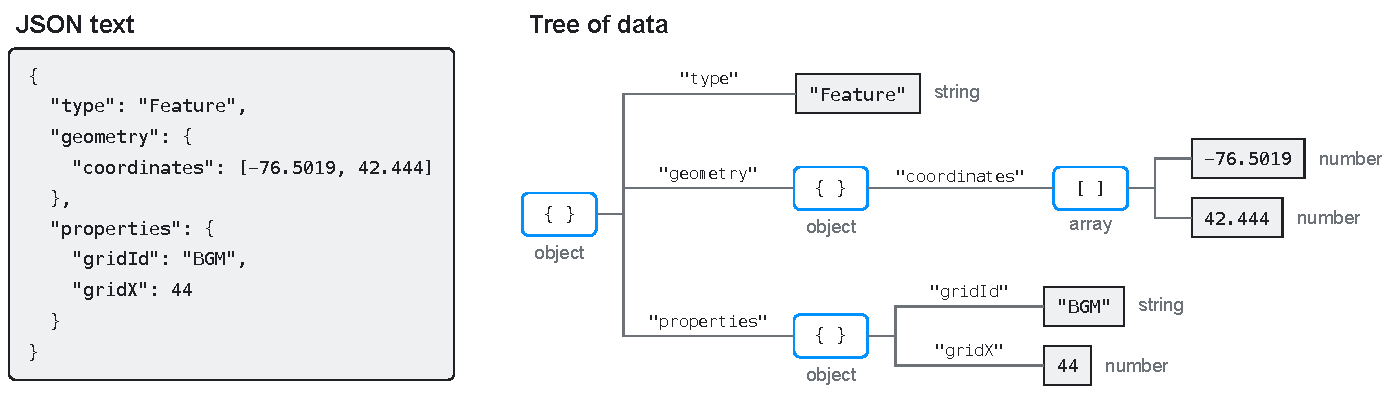
\includegraphics[width=\textwidth,height=0.44\paperheight,keepaspectratio]{assets/Fig-JSON-Tree.pdf}

  \vspace{0.6em}
  \raggedright
  We reach the grid identifier \code{"BGM"} by following the
  \code{"properties"} key and then the \code{"gridId"} key.
  \lecturesource{JSON: the tree figure and the paragraph on values.
    Figure: ../figs/Fig-JSON-Tree/Fig-JSON-Tree.pdf (light TikZ build).}
\end{frame}

\begin{frame}{RESTful Web Services}
  \hilite{Representational State Transfer (REST)} is an architecture for
  creating stateless web services: each request carries all the information
  that the server needs. REST organizes a web service around
  \hilite{resources}, items of data such as a user, an experiment, or a
  weather forecast. Each resource has its own URL.

  \vspace{0.5em}
  \centering
  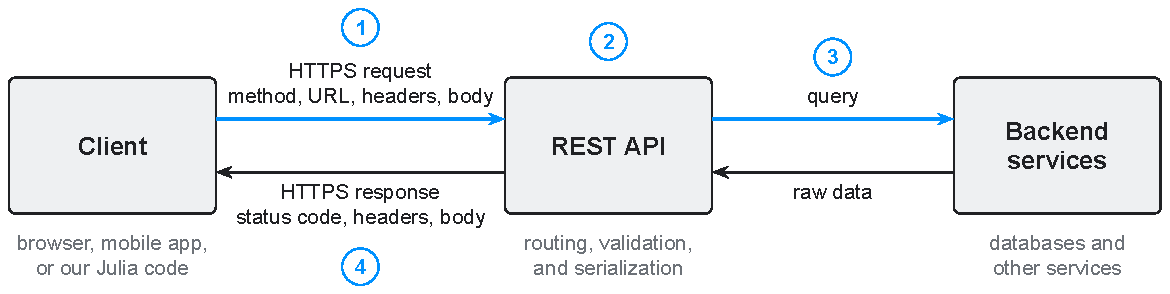
\includegraphics[width=\textwidth,height=0.42\paperheight,keepaspectratio]{assets/Fig-REST-Cycle.pdf}

  \vspace{0.5em}
  \raggedright
  A typical \hilite{RESTful} web service answers a request in four steps. The client
  needs to know what to send and what to expect in return.
  \lecturesource{RESTful Web Services: the definition, the resources paragraph, the request-response figure, and the paragraph after the four steps.
    Figure: ../figs/Fig-REST-Cycle/Fig-REST-Cycle.pdf (light TikZ build).}
\end{frame}

\begin{frame}{The Four Steps of the Cycle}
  \begin{enumerate}\setlength{\itemsep}{0.6em}
    \item \hilite{Client $\rightarrow$ REST API}: the client sends an HTTPS
      request to an endpoint. It selects the HTTP method, and encodes any data
      in the body, typically as JSON.
    \item \hilite{REST API internals}: the API maps the endpoint to a handler
      function (routing). The handler checks the client and its inputs
      (validation), parses the JSON in the request, and converts the result
      back into JSON (serialization).
    \item \hilite{REST API $\rightarrow$ backend services}: the handler gets
      data from a database or another web service, often with a protocol other
      than HTTP.
    \item \hilite{REST API $\rightarrow$ client}: the API converts the result
      into a JSON response, attaches a status code, and sends the response back
      over HTTPS.
  \end{enumerate}
  \lecturesource{RESTful Web Services: the four steps of the request-response cycle.}
\end{frame}

\begin{frame}{HTTP Methods and CRUD}
  Most of what a client does with a resource is one of four operations:
  \hilite{create}, \hilite{read}, \hilite{update}, or \hilite{delete}
  (\hilite{CRUD}). A RESTful API maps each operation onto an HTTP method.

  \vspace{0.4em}
  \centering
  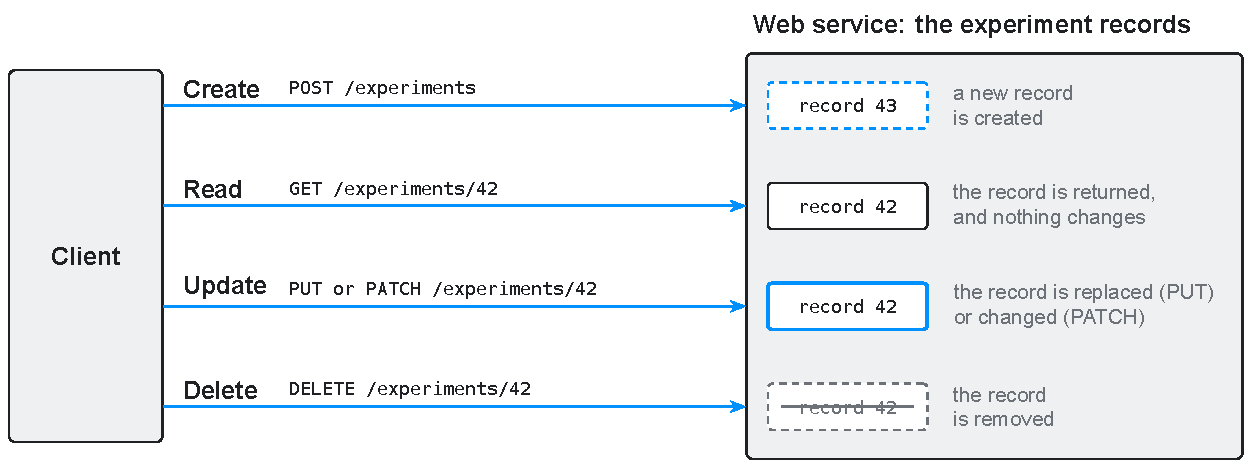
\includegraphics[width=\textwidth,height=0.50\paperheight,keepaspectratio]{assets/Fig-CRUD-Methods.pdf}

  \vspace{0.4em}
  \raggedright
  A lab runs a web service for its experiment records. A \code{GET} request
  leaves the records unchanged, and the other requests change them.
  \lecturesource{HTTP Methods and CRUD: the opening paragraph, the experiment records service, and the CRUD figure.
    Figure: ../figs/Fig-CRUD-Methods/Fig-CRUD-Methods.pdf (light TikZ build).}
\end{frame}

\begin{frame}{What the Server Does for Each Method}
  The URL \code{/experiments} is the collection of all the records. The URL
  \code{/experiments/42} is the record with identifier \code{42}.

  \vspace{0.3em}
  \centering
  {\footnotesize\setlength{\tabcolsep}{4pt}%
  \begin{tabular}{>{\raggedright\arraybackslash}p{0.11\textwidth}>{\raggedright\arraybackslash}p{0.27\textwidth}>{\raggedright\arraybackslash}p{0.35\textwidth}>{\raggedright\arraybackslash}p{0.17\textwidth}}
    \toprule
    \textbf{Operation} & \textbf{Example request} & \textbf{What the server does} & \textbf{Success code}\\
    \midrule
    Create & \code{POST /experiments} & creates a new record from the JSON in the body & \code{201 Created}\\
    \addlinespace[1.5pt]
    Read & \code{GET /experiments/42} & returns record \code{42}, and changes nothing & \code{200 OK}\\
    \addlinespace[1.5pt]
    Update & \code{PUT /experiments/42} & replaces record \code{42} with the JSON in the body & \code{200 OK}\\
    \addlinespace[1.5pt]
    Update & \code{PATCH /experiments/42} & changes only the fields that the body lists & \code{200 OK}\\
    \addlinespace[1.5pt]
    Delete & \code{DELETE /experiments/42} & removes record \code{42}, and returns no body & \code{204 No Content}\\
    \bottomrule
  \end{tabular}}
  \lecturesource{HTTP Methods and CRUD: the experiment records service and the CRUD table.}
\end{frame}

\begin{frame}{Safe and Idempotent Methods}
  \begin{itemize}\setlength{\itemsep}{0.6em}
    \item \hilite{Safe}: the method only reads data. Of the five methods, only
      \code{GET} is safe.
    \item \hilite{Idempotent}: sending the same request many times has the
      same effect on the server as sending it once. \code{GET}, \code{PUT},
      and \code{DELETE} are idempotent.
    \item \code{POST} is not idempotent: in our example, sending the same
      \code{POST} request twice creates two records.
  \end{itemize}

  \vspace{0.5em}
  A client can send an idempotent request again after a timeout.
  \lecturesource{HTTP Methods and CRUD: safe and idempotent methods and the timeout paragraph.}
\end{frame}

\begin{frame}{Why Are RESTful Web Services so Popular?}
  RESTful web services have become the standard for building web APIs. Three
  principles of the architecture explain why:

  \vspace{0.4em}
  \begin{itemize}\setlength{\itemsep}{0.6em}
    \item \hilite{Statelessness}: each request is complete on its own, and
      the server does not need to remember earlier requests from the client.
      Any one of many servers can answer the next request.
    \item \hilite{Uniform interface}: a small, well-known set of methods
      operates on resource URLs. A developer who has used one RESTful API can
      quickly understand another.
    \item \hilite{Layered system}: the client does not need to know whether it
      is talking to a single program or to a chain of services. The developers
      can change the backend without changing the client.
  \end{itemize}
  \lecturesource{Why Are RESTful Web Services so Popular?: the three principles.}
\end{frame}

\begin{frame}{Example: The National Weather Service API}
  In this example, we write a small Julia library, called a software
  development kit (SDK), and download the hourly forecast for Ithaca, NY:

  \vspace{0.5em}
  \begin{enumerate}\setlength{\itemsep}{0.5em}
    \item Build the URL of the points endpoint from a latitude and longitude,
      and make an HTTP GET call.
    \item Read the URL of the hourly forecast from the response, and call the
      forecast endpoint.
    \item Pass a handler to the forecast call that returns the forecast as a
      table.
  \end{enumerate}

  \vspace{0.5em}
  The NWS API publishes resources that a client can read but not change. Every
  call in the example uses the \code{GET} method.
  \slidenote{Example:}{\href{\examplelink}{A software development kit for the National Weather Service API}}
  \lecturesource{Why Are RESTful Web Services so Popular?: the example box. HTTP Methods and CRUD: the read-only paragraph. Companion example: Tasks 1--3.}
\end{frame}

\begin{frame}{Summary}
  We introduced web services, the HTTP messages that carry their calls, and
  the REST architecture.

  \vspace{0.5em}
  {\large\textbf{\ink{Key takeaways}}}
  \vspace{0.3em}
  \begin{itemize}\setlength{\itemsep}{0.6em}
    \item \textbf{\ink{Web services and APIs.}} A client needs to know what to
      send to an endpoint and what to expect in return.
    \item \textbf{\ink{HTTP requests and responses.}} A request has a method,
      a URL, headers, and a body. The status code of the response says whether
      the request succeeded.
    \item \textbf{\ink{REST and the CRUD methods.}} Each resource has its own
      URL, and POST, GET, PUT or PATCH, and DELETE create, read, update, and
      delete it.
  \end{itemize}

  \vspace{0.5em}
  These ideas are the foundation for calling any web service from our own code.
  \lecturesource{Summary: three key takeaways and the closing sentence.}
\end{frame}

\end{document}
